\documentclass[11pt]{article}
\usepackage{../ps1/classTools}
\usepackage{listings}
\usepackage{graphicx}

\begin{document}

% To include a problem set header, use the psHeader command
\psHeader{2}{Wed Sep. 21, 2022 (11:59pm)}

\textbf{Your name: Nikhil Datar}

\textbf{Collaborators: Dhrub Singh, John Rho}

\textbf{No. of late days used on previous psets: 0}

\textbf{No. of late days used after including this pset: 0}
\\

Please review the Syllabus for information on the collaboration 
policy, grading scale, revisions, and late days.


\begin{enumerate}
     \item  (reductions) The purpose of this exercise is to give you practice formulating reductions and proving their correctness and runtime.
    Consider the following computational problem:

    \compprob{AreaOfConvexPolygon()}
    {Points $(x_0,y_0),\ldots,(x_{n-1},y_{n-1})$ in the $\R^2$ plane that are the vertices of a convex polygon (in an arbitrary order) whose interior contains the origin}
    {The area of the polygon formed by the points}


    \begin{enumerate}
        \item \label{part:polar} 
        Show that AreaOfConvexPolygon$\leq_{O(n),n}$ Sorting.  Be sure to analyze both the correctness and runtime of your reduction.

        In this part and the next one, you may assume that a point $(x,y)\in \R^2$ can be converted into polar coordinates $(r,\theta)$ in constant time. 
        \\\\
        You may find the following useful:
        \begin{itemize}
            \item The polar coordinates $(r,\theta)$ of a point $(x,y)$ are the unique real numbers $r\geq 0$ and $\theta\in [0,2\pi)$ such that $x=r\cos \theta$ and $y=r\sin \theta$. Or, more geometrically, $r=\sqrt{x^2+y^2}$ is the distance of the point from the origin, and $\theta$ is the angle between the positive $x$-axis and the ray from the origin to the point.
            \item The area of a triangle is $A = \sqrt{s(s-a)(s-b)(s-c)}$ where $a, b, c$ are the side lengths of the triangle and $s = \frac{a + b + c}{2}$ (\href{https://en.wikipedia.org/wiki/Heron\%27s_formula}{Heron's Formula}).
        \end{itemize} \\
        
        Let us treat this as a reduction between two computational problems. By a reduction, we can show tha solving the computational problem AreaOfConvexPolygon is the same as solving the computational problem the Sorting Problem. 
        Suppose we define the algorithm AreaofConvexPolygon as follows: \\
        
        \begin{enumerate}
            \item Convert all points to their polar form $(r, \theta)$. That is, make all $(x_i, y_i) = (r_i, \theta_i) \forall i=0, 1, \dots, n-1$. 
            \item Then, create (key, value) pairs $(K_i, V_i) = (\theta_i, r) \forall i=0, 1, \dots, n-1$, where the $\theta 's$ are the keys, and the $r's$ are the values. 
            \item Sort the points $(K_0, V_0), (K_1, V_1), \dots, (K_{n-1}, V_{n-1})$, using MergeSort, based on the keys (which again are the $\theta 's$ defined in the previous step), and then store the resulting array. Thus the resulting array should be some order of pairs $(\theta_i, r_i)$.
            
            \item Create a running sum initialized to 0. For every two adjacent points in the sorted list (where we count the first and last points as adjacent), define a triangle, where the vertices of the triangle are the the two adjacent points along with the origin. For example, if we have sorted points $(r_0, \theta_0), (r_1, \theta_1) \dots, (r_{n-1}, \theta_{n-1})$, then the pairs we would consider would be $\left(\{(r_0, \theta_0), (r_1, \theta_1)\}, \{(r_{1}, \theta_{1}), (r_{2}, \theta_{2})\}, \{(r_{n-2}, \theta_{n-2}), (r_{n-1}, \theta_{n-1})\}\right)$ along with the origin for all the pairs.\\
            
            Let the sides of the triangle formed be the lengths $x, y, z$. Suppose we are dealing with the triple $(\theta_j, r_j), (\theta_k, r_k), (0,0)$ respective to $x, y, z$. Then we have $x=r_j$, $y=r_k$, and we find $z$ using the Law of Cosines. That is, $z = x^2 + y^2 - 2xycos(\theta_k - \theta_j)$. We then can find the area of the triangle with all the sides calculated using Heron's formula. In particular, we first calcualte the semi-perimeter $s = \frac{x+y+z}{2}$ and then find the area $A$ by calculating $A = \sqrt{s(s-a)(s-b)(s-c)}$. Now, add this sum to the running sum, such that by the end of calculating all the areas of the triangles individually the sum is the sum of all the individual triangle areas. 
            
            
            \item Return the sum calculated in the previous step and report this area as the area of the convex polygon. 
        \end{enumerate} \\
        
        \textbf{Correctness: }Let us start by proving correctness of the algorithm. After conversion to polar coordinates, the algorithm sorts based on $\theta$. We can treat this sorting as a black-box oracle, and assume correctness (suppose we have access to an aglorithm) Indeed, this would give us the points in the correct order to continue to the next step, because in polar coordinates $\theta$ represents the angle starting at the positive $x-axis$, going left, and stopping at the line segment formed by the point and the origin. \\
        
        Then, let us consider the step which actually calculates the areas of the triangles. Importantly, we have that the convex polygon contains the origin. This allows us to extend and create a segment from all points to the origin, which is why we are able to create distinct triangles containing the origin. Then, when we form all triangles using adjacent points, we will end up traveling around the full $0 \to 2\pi$ of the Cartesian plane. Then, because we are considering all two adjacent points in the sorted list, we ensure we iterate through all possible distinct triangles generated. 
        
        \textbf{Runtime: } Let us consider the runtime at each of the steps.
        
        \begin{enumerate}[i]
            \item At the first step, we convert all the points to the polar form. Each conversion takes constant time, and we perform the conversion on $n$ points. Thus, this step can be considered $O(n)$ time. 
            \item At the next step, we again convert the pairs to (k,v) pairs. Again, this is like the previous step and takes $O(n)$ time. 
            \item We then sort the points using the best sorting algorithm such as MergeSort as an oracle. We make $O(1)$ call to this oracle.
            \item In the next step, we are calculating the areas generated by the triangles formed by the $n$ points. The area calculations themselves are constant time, but performed on triangles generated by the $n$ points results in $O(n)$ runtime at this step.
            \item This step is simply returning a value and thus is $O(1)$.
            
        \end{enumerate}\\
        
        Analying the above runtimes, we see that the maximum runtime of the above steps is $O(n)$. Since we treated the Sorting problem as a black-box oracle, we thus can say, as desired, that using a reduction from the Area computational problem to the Sorting computational problem, AreaOfConvexPolygon$\leq_{O(n),n}$ Sorting.
        
        \item Deduce that AreaOfConvexPolygon can be solved in time $O(n\log n)$.
        
        From the previous step, we saw that when we treating the Sorting oracle as $O(1)$, the runtime of the reduction was $O(n)$. Thus, the runtime of complete algorithm can be thought of as the sum of runtimes of the reduction and oracle calls. Since we have one call of size $n$ to an oracle call that runs in time $O(n \times \log n)$, we have that the runtime of AreaOfConvexPolygon is $O(n + n \times \log(n))$, which simplifies to $O(n \times \log n)$. 


        \item Let $\Pi$ and $\Gamma$ be arbitrary computational problems, and suppose that there is a reduction from $\Pi$ to $\Gamma$ that runs in time at most $g(n)$ and makes at most $k(n)$ oracle calls, all on instances of size at most $f(n)$.  Show that if $\Gamma$ can be solved in time at most $T(n)$, then $\Pi$ can be solved in time at most $O(g(n)+k(n)\cdot T(f(n)))$. Note that the case $k(n)=1$ was stated and proved in class; the case $k(n)>1$ is useful as well, such as in Part~\ref{part:nopolar} below.  \\
        
        Suppose we have the computational problems $\Pi$ and $\Gamma$. Then suppose we have an algorithm $A$ that solves $\Pi$ with a single call to an oracle, and algorithm $A'$ that solves $\Gamma$. We define $A'$ as an algorithm that takes time $T(n)$ for inputs size $n$ to solve $\Gamma$. It then follows that by the rules of reduction, that the runtime of algorithm $A$ is the runtime of the reduction (suppose $g(n)$), where we treat oracle calls as constant) and the runtime of an algorithm that solves the oracle, in this case $A'$. Suppose the input to $A'$, the oracle, is $f(n)$. Then it follows that the runtime for the algorithm is simply $O(g(n) + 1 \times T(f(n)))$. This has already been solved as shown in class. Now, we extend this argument for an algorithm $A$ that makes $k(n)$ calls to an oracle $A'$. Using the same logic as before (where the overall runtime is the sum of the reduction runtime and the oracle call runtime), we find that the runtime for $A$ in this case is $O(g(n) + k(n) \times T(f(n))$.
        
        \item (*challenge; extra credit) Come up with a way to avoid conversion to polar coordinates and any other trigonometric functions in solving AreaOfConvexPolygon in time $O(n\log n)$.  Specifically, design an $O(n)$-time reduction that makes $O(1)$ calls to a Sorting oracle on arrays of length at most $n$, using only arithmetic operations $+$, $-$, $\times$, $\div$, and $\sqrt{\hspace{1em}}$, along with comparators like $<$ and $==$.  (Hint: first partition the input points according to which quadrant they belong in, and consider $\tan\theta$ for a point with polar coordinates $(r,\theta)$.) \label{part:nopolar}
        \end{enumerate} \\
        
        Suppose we define an algorithm as follows: 
        \begin{enumerate}[i]
            \item First sort each point $(x_i, y_i) \forall i=0, 1, \dots, n-1$ into 1 of 4 bins, or lists, based on which quadrant the point lies within in the Cartesian plane.
            \item Then, consider (find) the value $\frac{y}{x}$ for each of these points, separately for each of the 4 lists. This value is equal to $\tan \theta$
            \item Now with those values considered, sort the points within each of the 4 quadrant lists based on the values. Join the 4 arrays based on these sorted values, in order from the list referring to the first quadrant, then second quadrant, then third quadrant, then fourth quadrant. 
            \item Compute the area using a technique similar to described in part $a$ with Heron's formula. We can subdivide and consider the triangle formed by the origin and every adjacent pair of points within the complete sorted list, just like before. For each of these triangles, we can find the side lengths by using the distance formula between each pair of the 3 points. For any pair of points $(x_j, y_j), (x_k, y_k)$, the distance between the points (and side length of the triangle being considered) would be $d = \sqrt{(x_j - x_k)^2 + (y_j - y_k)^2}$. Once we calculate all of these sizes, we use Heron's formula to calculate the area of the triangle. Using a running sum, we can calculate the total area of the polygon by summing the area of these individual triangles. 
            \item Return the sum as the area of the polygon
        \end{enumerate} \\
        
    \textbf{Correctness: } This algorithm is similar to 1a. The main challenge with not converting to polar coordinates deals with sorting the points in the first place. Consider the steps taken to sort. We first partition the points into lists depending on the quadrant where the point lies (we have 4 total lists). This can simply be completed by observing the point itself. Next, we sort every quadrant list based on the value of $\frac{y}{x}$ for every point $(x, y)$, because this is equal to $\tan \theta$. This works because tangent is a monotonically increasing function within each intervals of $-\frac{\pi}{2} \to \frac{\pi}{2}$ and such (other than the asymptotes). Thus, since the points within each quadrant all have the same sign ($-$ or $+$) for the value $\frac{y}{x}$ for each point, they can be sorted accordingly. Then, once we join the 4 separate lists in the order prescribed in the algorithm, we can ensure that they are in order, just like how we used $\theta$ values in $1a$. Then, the rest of the proof with the triangle areas follows from above in $1a$. 
    
    \textbf{Runtime}: We will analyze each of the steps of the algorithm to determine the overall runtime. 
    
    \begin{enumerate}[(i)]
        \item Partitioning the going simply means running through all the points and assigning accordingly, so this step takes $O(n)$ time.
        \item Again calculating a particular value for all $n$ points should take $O(n)$ time. 
        \item This step makes $O(4)$ calls to a sorting oracle (such as MergeSort) in order to sort each of the 4 quadrant lists. Thus, we have made a constant set of calls to the oracle.
        \item Computing the area is done in constant steps for each of the triangles formed by the $n$ points. Thus, the runtime of this step is $O(n)$. 
        \item Returning is done in constant time $O(1)$.
    \end{enumerate}
    
    All the above steps considered, we can see that the reduction from AreaOfConvexPolygon to Sorting can be done in $O(n)$ with $O(1)$ time calls to a sorting oracle like mergeSort, because that is the maximum runtime of an individual step. 
    
    
    Similar techniques to what you are using in this problem are used in algorithms for other important geometric problems, like finding the Convex Hull of a set of points, which has applications in graphics and machine learning.
    
    \newpage

    
    \item (augmented binary search trees) The purpose of this problem is to give you experience reasoning about correctness and efficiency of dynamic data-structure operations, on variants of binary-search trees. 
    
    Specifically, we will work with {\em selection data structures}.
    We have seen how binary search trees can support min queries in time $O(h)$, where $h$ is the height of the tree.  A generalization is {\em selection} queries, where given a natural number $q$, we want to return the $q$'th smallest element of the set.  So $\texttt{DS.select(0)}$ should return the key-value pair with the minimum key among those stored by the data structure $\texttt{DS}$, $\texttt{DS.select(1)}$ should return the one with the second-smallest key, $\texttt{DS.select(n-1)}$ should return the one with the maximum key if the set is of size $n$, and $\texttt{DS.select((n-1)/2)}$ should return the median element if $n$ is odd.
    
    In the Roughgarden text (\S11.3.9), it is shown that if we {\em augment} binary search trees by adding to each node $v$ the size of the subtree rooted at $v$, then Selection queries can be answered in time $O(h)$.\footnote{Note that the Roughgarden text uses a different indexing than us for the inputs to Select. For Roughgarden, the minimum key is selected by Select(1), whereas for us it is selected by Select(0).}
    
    \begin{enumerate}
        \item In the Github repository, we have given you a Python implementation of size-augmented BSTs supporting search, insertion, and selection, and with a stub for \texttt{rotate}. One of the implemented functions (\texttt{search}, \texttt{insert}, or \texttt{select}) has a correctness error, and another one is too slow (running in time linear in the number of nodes of the tree rather than in the height of tree). Identify and correct these errors. You should provide a text explanation of the errors and your corrections, as well as implement the corrections in Python. \\
        
        The function that had a correctness error was \texttt{select}. The error was in the fact that the recursive call if the index is larger than the size of the left child was incorrect. This is because if we want to find the $k^{th}$ smallest element, then if it is on the right side of the tree, we simply cannot make the recursive call to search with $k$ as the input, because now we are only considering the right half of the tree, in which all nodes are larger than the left side of the tree. Thus, we must adjust the input index whenever we determine it would be found on a right child of the node currently being observed. This resulted in the change of calling search with the index (ind - left-size - 1). \\
        
        The other error, which was with runtime, was with \texttt{insert}. This was because of the fact that the function originally called calculate-sizes at the end of the function in order to update the sizes, which takes $O(n)$ time rather than $O(h)$. The change implemented is changing the size as we iterate through the tree checking where the key should be inserted. Since every tree we go through is ultimately going to have the key added as a descendant, we can increment the current node size by 1. This meant incrementing the size of the node currently on right before making a recursive insert call either when the key is to be inserted on the left child or right child. 
        
        
        \item Describe (in pseudocode or pictures) how to extend \texttt{rotate} to size-augmented BSTs, and argue that your extension maintains the runtime $O(1)$. Prove that your new rotation operation preserves the invariant of correct size-augmentations. (That is, if every node's size attribute had the correct subtree size before the operation, then the same is true after the operation). 
        
        \begin{enumerate}
            \item First we consider which child the rotation is being performed on. This information is given to us by the parameters of the rotate function, which tells on which side the child is being rotated (right or left). 
            \item Now, we must consider the effects of the rotation on the new child of the root node (self). If performing a left rotation, then the right child of the child of the root will be the new child of the root. However, if performing a right rotation, then the opposite is true; it will be the left child of the child identified in the previous step that will become the new child of the root in the direction identified in the previous step. 
            \item Meanwhile, the original child will be rotated to become the child of its previous child that is now the child of the root (or, more clearly, the sub-child we identified in the previous step). The original child is now the child of its previous child in the same direction as the rotation. 
            \item The last node that is switched is the child of the node that is now the child of the root node (the child of the original root's child's child, in directions addressed above) that is in the direction of the rotation. This now becomes the child of the original node that got rotated (child of the root) in the direction opposite the rotation. This completes the rotations of the trees. \\
            
            These rotations will be easier conveyed as a diagram:
            
            However, we still have not updated the size components. Note that the size of the new child of the root node has gained as a descendant its parent as well as the descendants in the opposite direction. However, it also loses it's original child in the direction of the rotation. Thus, the original size of this node will need to be updated accordingly, where the size is updated to be the previous size plus the size of the parent's descendants minus the child lost plus 1 (for the parent). \\
            
            Meanwhile, the original parent moved lost the entire descendants on the side which the child was rotated to become the new child of the root, but gained that child's previous child. Thus, we must adjust the size accordingly. This can be done by storing the necessary size components described herein before performing any operations. We then update the particular nodes described in the paragraph by adjusting the nodes based on which subtrees were added as children and which were removed, giving us the final sizes. \\ 
            
            We can prove correctness of this algorithm based on the fact that the rest of the tree remains the same and does not switch children. In particular, only the nodes described in the previous paragraph(s) that actually are switched are the ones where the size must be updated. Furthermore, the rotations themselves are correct, as illustrated by the diagrams below. They preserve the BinarySearchTree properties of every left being less than its parent and every right node being greater than its parent. Furthermore, we we again do not need to update the sizes of the nodes that do not gain or lose children from the rotation operations performed. \\
            
            Now let us consider the runtime of the algorithm. Note that the rotation operations described in the pseudocode are completely independent of the size of the BST. When we identify which node to rotate, which of its children will take its place, and which child of the original child's child will be switched, we are simply considering only 3 nodes that are switched every time (given these nodes exist) and the operations required to do so. Thus, the rotation algorithm completely would take $O(n)$ time. 
            
            While pseudocode may suffice, these size augmentation changes will be easier conveyed as diagrams. Below, I have attached diagrams for each of the four rotation - child combos. \\
            
            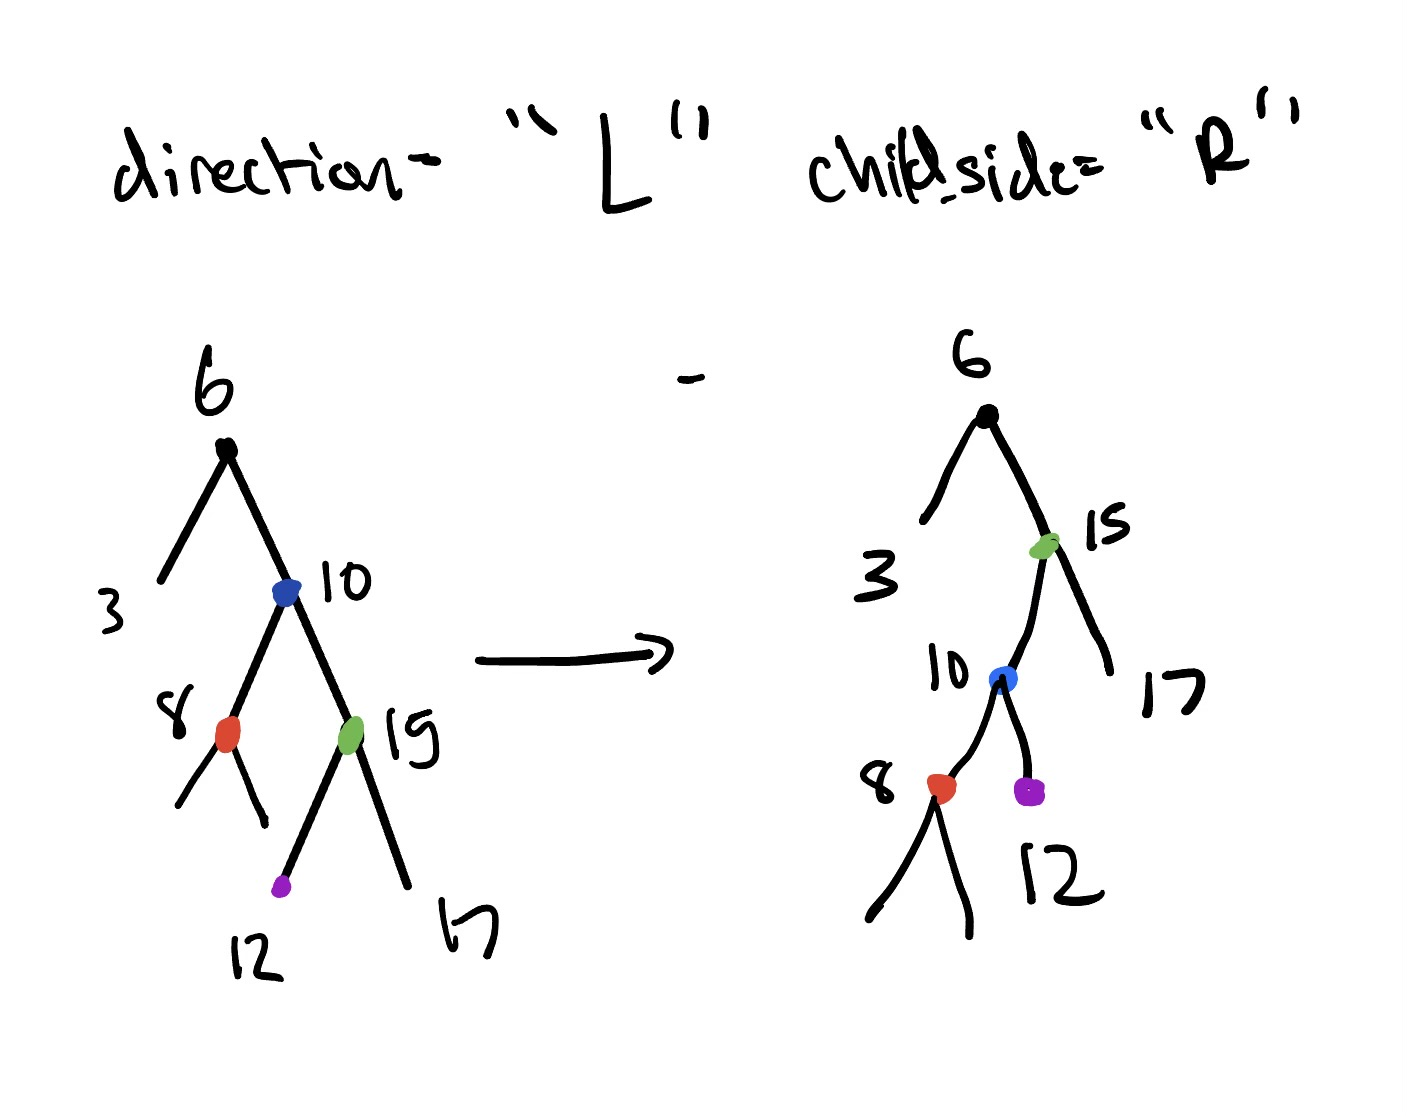
\includegraphics[width=0.75\textwidth]{./IMG_0001.jpg}\\
            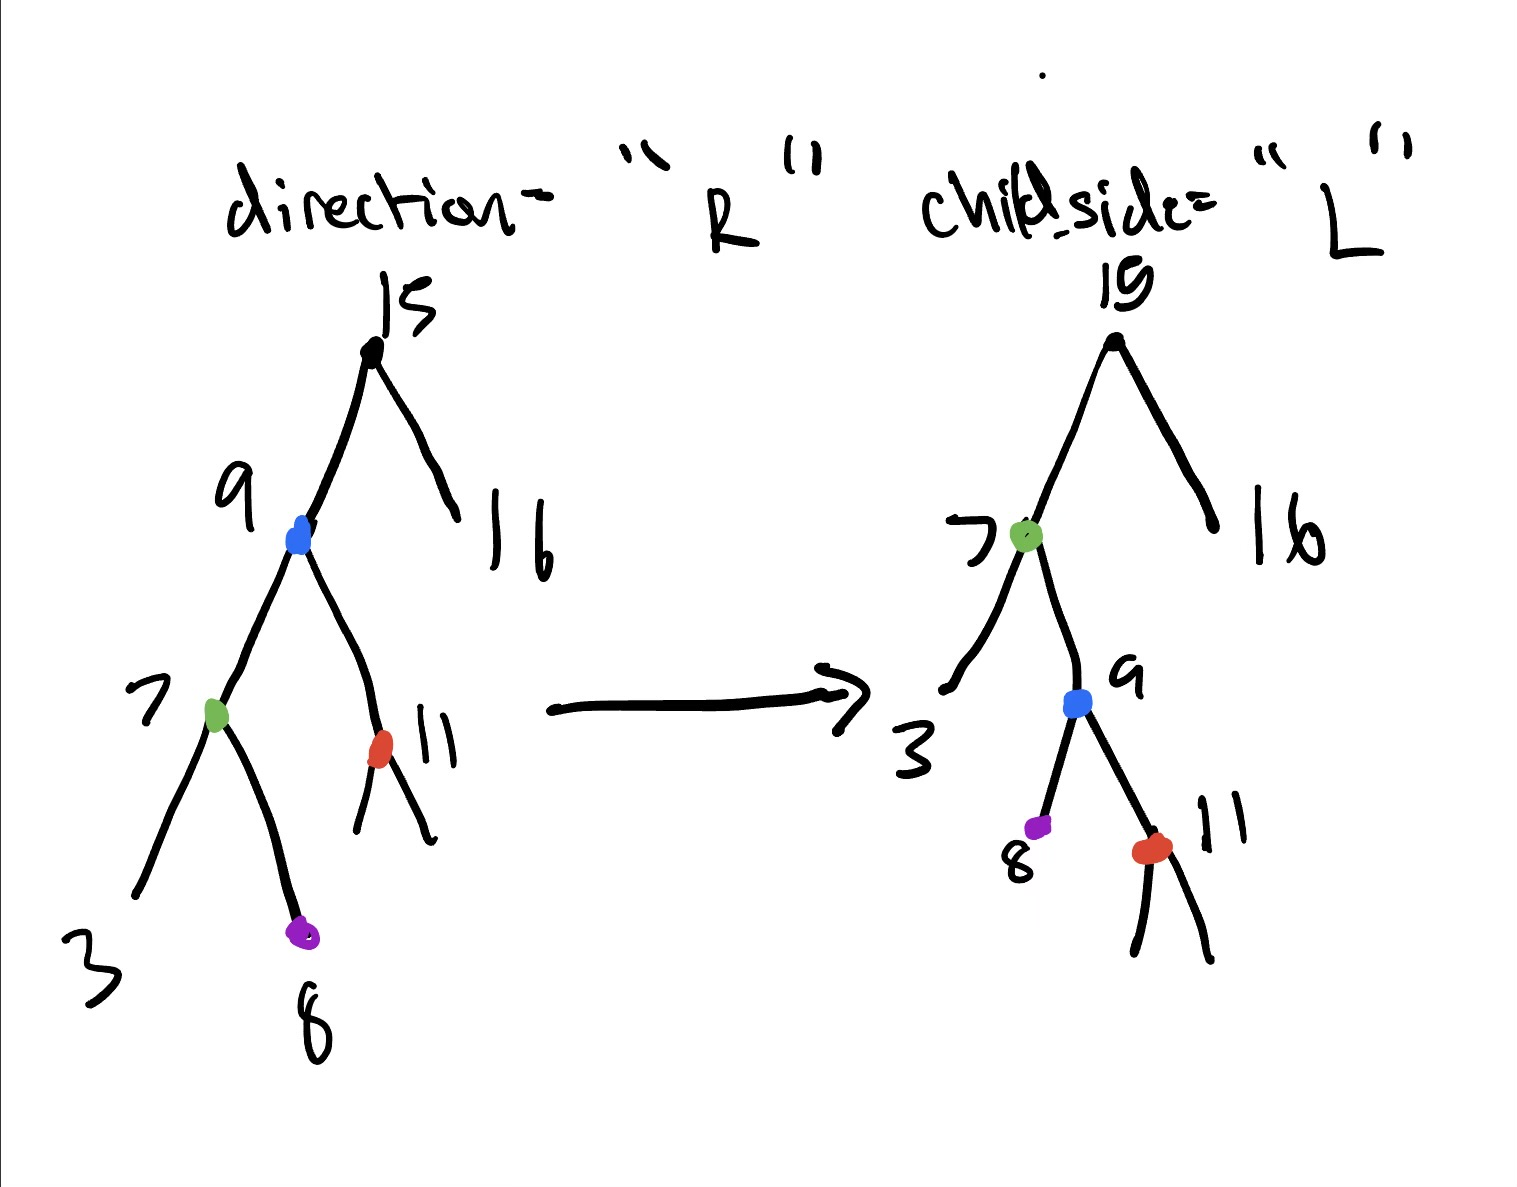
\includegraphics[width=0.75\textwidth]{./IMG_0002.jpg}\\
            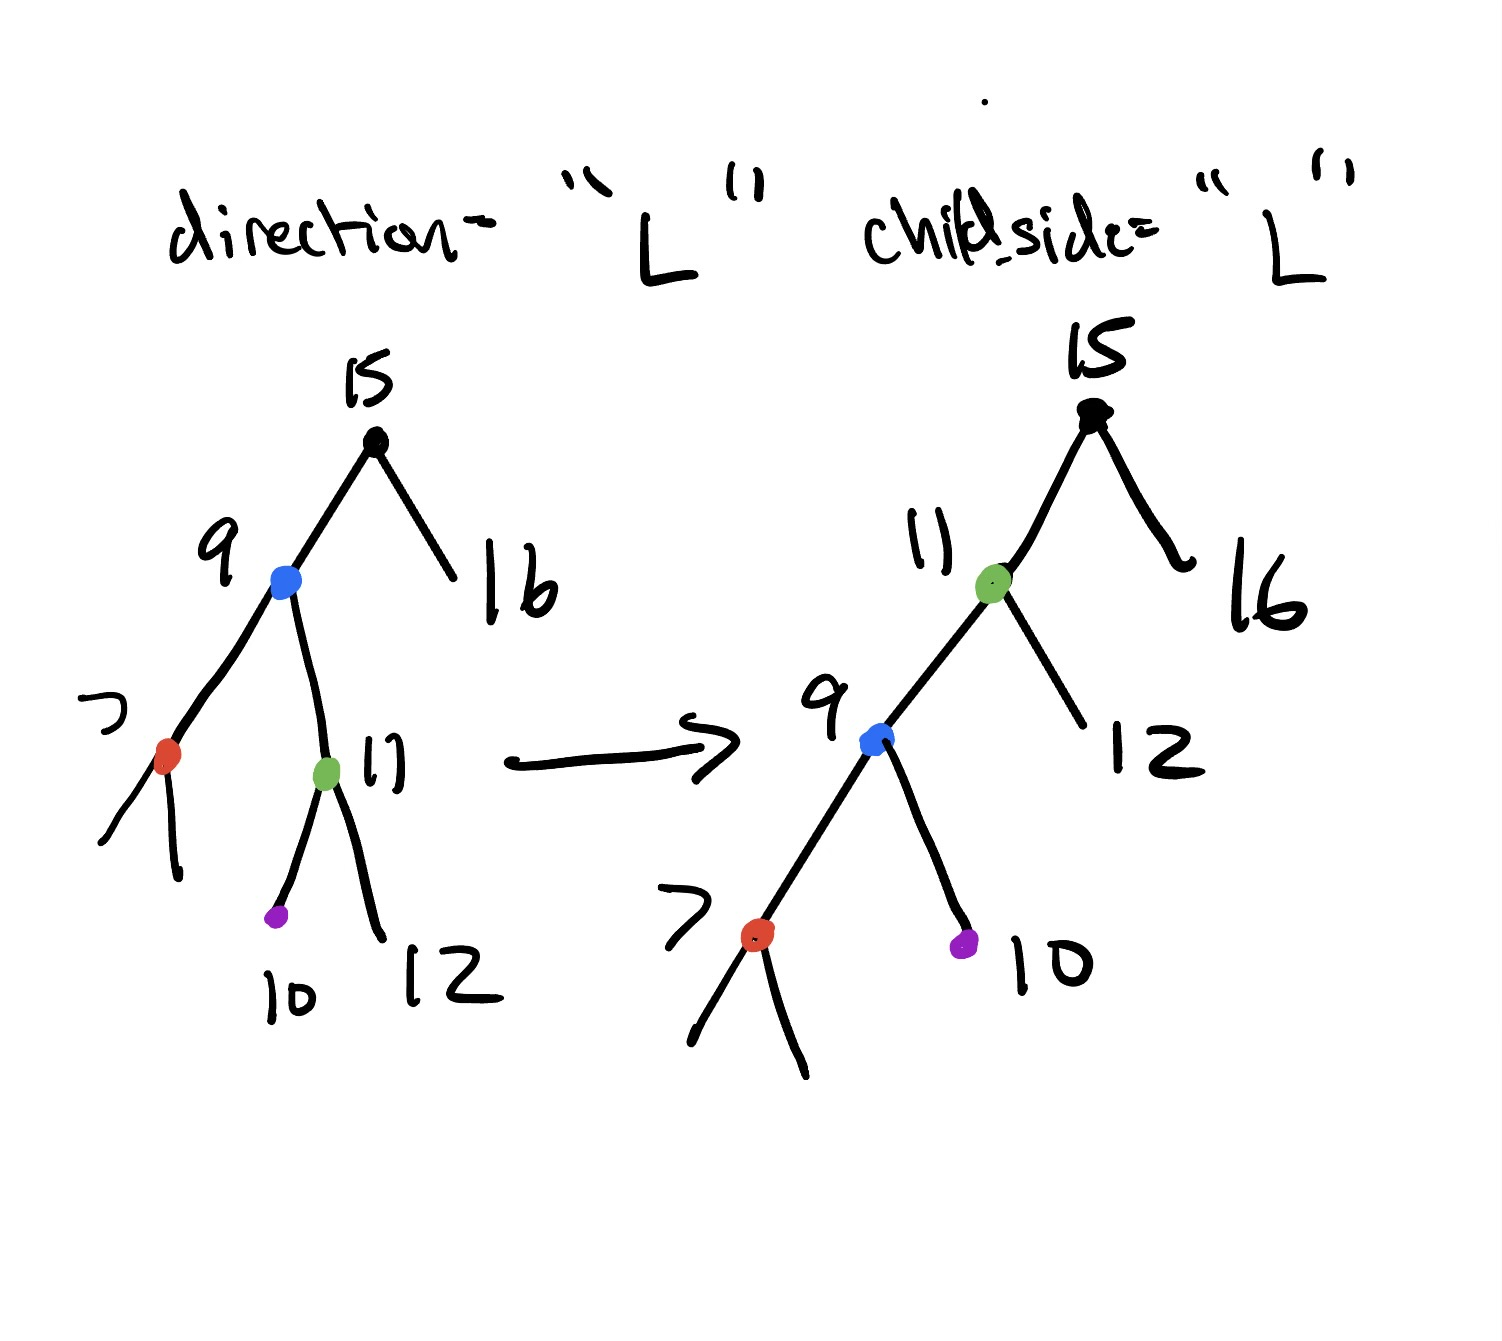
\includegraphics[width=0.75\textwidth]{./IMG_0003.jpg}\\
            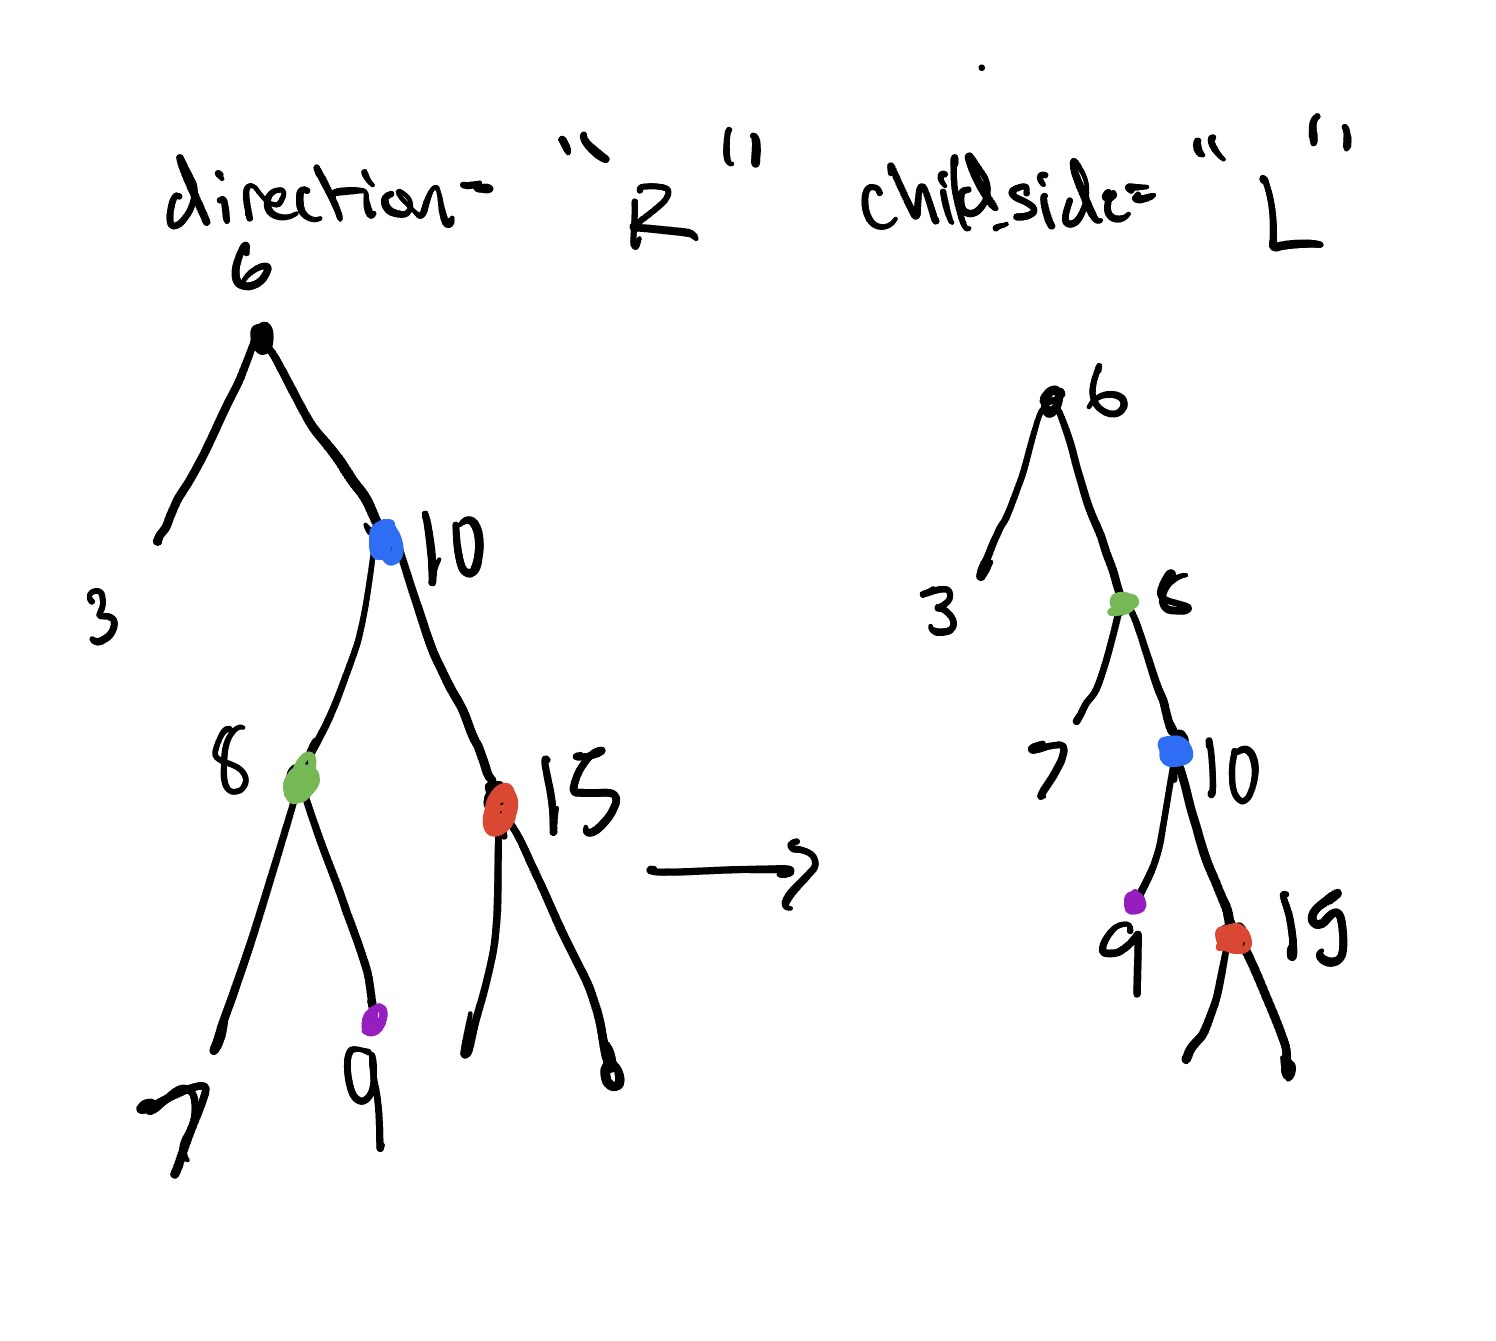
\includegraphics[width=0.75\textwidth]{./IMG_0004.jpg}\\
            
            The diagrams above show the rotations as described in the pseudocode. Following the colors and keys labeled at each node, it becomes clearer how a tree would be rotated given a direction and child side. I chose to make the blue node the child being rotated, a green node the node replacing this child, the red node the child of the original child node being rotated, and then purple the node that switches to become the child of this original child being rotated. This is consistent across the 4 diagrams. 
            
        \end{enumerate}
        
        \item Implement \texttt{rotate} in size-augmented BSTs in Python in the stub we have given you.
    

    \end{enumerate}
    
    \emph{Food for thought (do read - it's an important take-away from this problem):} This problem concerns size-augmented binary search trees. In lecture, we discussed AVL trees, which are balanced binary search trees where every vertex contains an additional \textit{height} attribute containing the length of the longest path from the vertex to a leaf (height-augmented). Additionally, every pair of siblings in the tree have heights differing by at most 1, so the tree is height-balanced. Note that if we augment a binary search tree both by size (as in the above problem) and by height (and use it to maintain the AVL property), then we create a dynamic data structure able to perform \texttt{search}, \texttt{insert}, and \texttt{select} all in time $O(\log n)$. 


\end{enumerate}



\end{document}
